\subsection*{a}
This result can be explained by means of the nuclear shell model. According to this model each sub-level of the nucleus can be identified by 4 quantum numbers $\{n, j, l, m_l\}$. For fixed $\{n, j, l\}$ 
one has that the $2l+1$ sub-levels given by $m_l = -l, -l+1, \dots, l-1, l$ are degenerate and each of this sub-levels can contain two nucleons with different spin z-projrection ($m_s = \pm 1$). \\
At first one can notice that if one sub-shell is filled with two nucleons (of the same type) then the spin contibution of that sub-shell is 0. Having an even number of protons and neutrons means that 
they combine in couples in the sub-shell in a way such that the contribution to the spin of each sub-shell is 0. \\
For what concerns the parity, each particle in the nucleus gives a contribute of $(-1)^l$ (the intrinsic parity of the nucleons is $+1$) and the total parity is the product of single parities. 
The product of the parities of two protons (neutrons) in the same sub-shell is always $+1$ since they, in particular, share the same quantum number $l$. Hence it is legitimate to expect an even-even nucleus
to be in the state $0^+$.
\vspace{10pt} \\
\centerline{\textbf{Answer}: spin $0$, parity $+$}.

\subsection*{b}
The process is governed by the strong interaction, hence quark flavour numbers and baryon numbers must be conserved.
By observing the final state it is immediate to see that the flavour number is 0, and the same holds for the barion numberm hence the
hadron must be a meson. \\
By looking at the \href{https://en.wikipedia.org/wiki/Meson#List}{table} of the allowed mesons one can conclude that the isospin $I$ must be either $0$ or $1$. 
On the other side in the final state $I_3=0$ and because of isospin components conservation law one concludes that $I_3=0$ also for the decaying pion.
In conclusion the admitted couples $(I, I_3)$ of isospins are $(0, 0), \ (1, 0)$.

\subsection*{c}
The nuclear potential is charge independent, in the sense that protons and neutrons feel the same potential. It is repulsive for very short distances and attractive for longer dstances (but the force range is short).
In addition a proton feels the effect of the Coulomb interaction with the nucleus, a factor that does not affect the neutron since it is electric neutral.
\begin{figure}[h]
    \centering 
    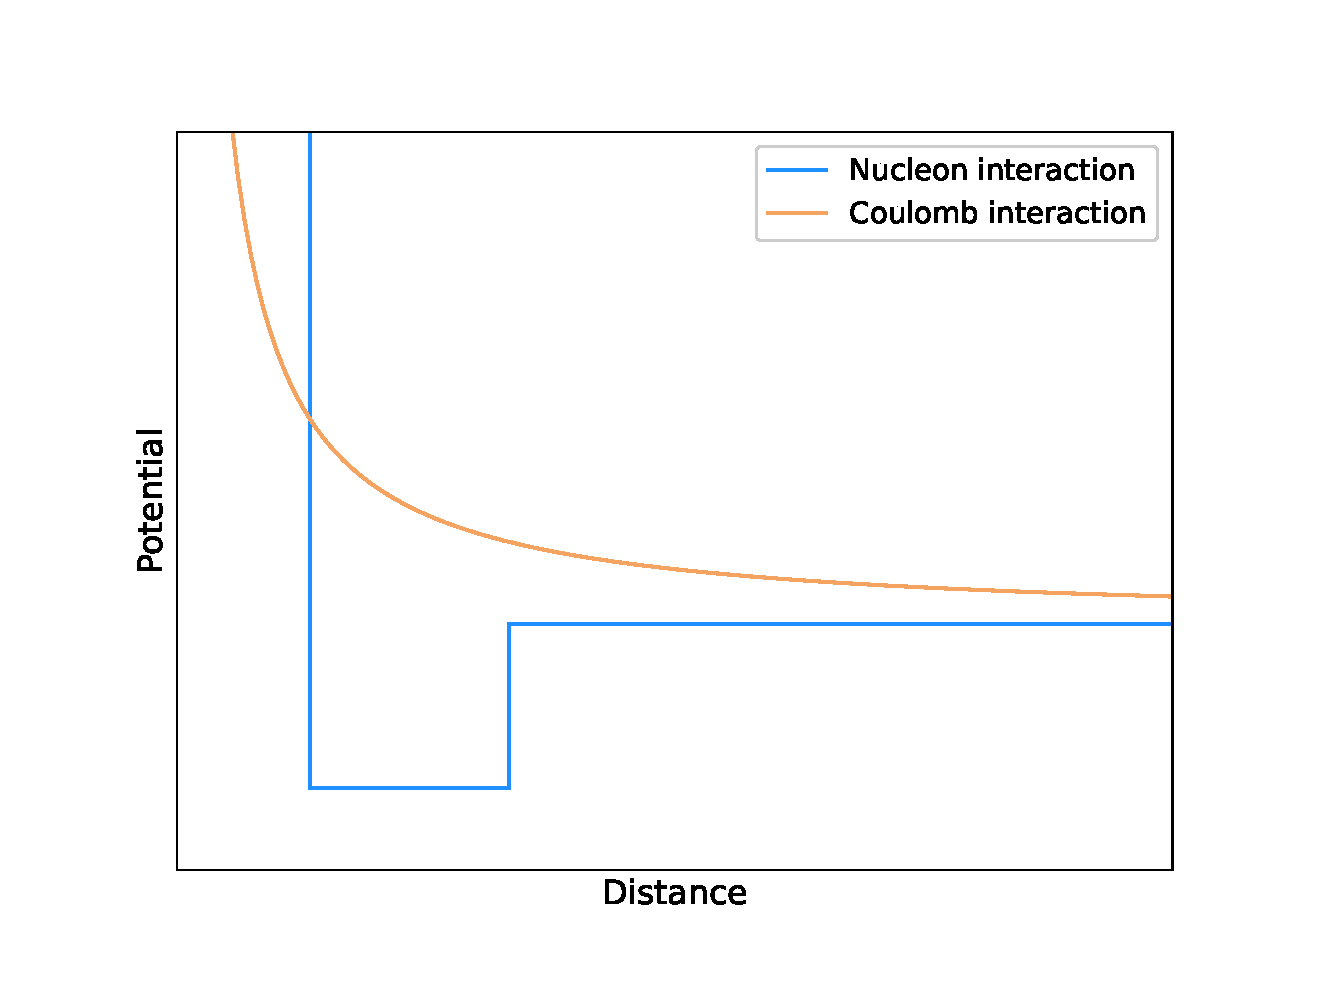
\includegraphics[scale=0.4]{ex1/nucleons.eps}
    \caption{Nucleons interaction. The plot reports  a simplified model of the nuclear potential between two nucleons (blue) and the Coulomb repulsion (orange) which is present
    only for the proton. The plot is purely qualitative and not in scale.}
\end{figure}

\subsection*{d}


\subsection*{e}
The energy to steal a neutron can be calculated by computing the difference between the binding energy $B(A, Z)$ before and after the removal (see exercise 2b for more details). 
\begin{enumerate}
    \item $^{118}Sn \rightarrow B(118, 50) - B(117, 50) \approx 9.03 MeV/c^2$
    \item $^{16}O \rightarrow B(16, 8) - B(15, 8) \approx 15.80 MeV/c^2$
    \item $^{119}Sn \rightarrow B(119, 50) - B(118, 50) \approx 6.54 MeV/c^2$
\end{enumerate}
hence it is harder to steal a neutron from $^{16}O$.

\subsection*{f}
The number of events $N$, the luminosity $\mathcal{L}$ and the cross section $\sigma$ are connected trough the relation
\begin{equation*}
    N = \sigma L
\end{equation*}
and the correct number of events, that is the value that takes account of the efficency $\epsilon$ of the detector and of the backround events number $N_{back}$, is
\begin{equation*}
    N = \frac{N_{obs} - N_{back}}{\epsilon}
\end{equation*}
so that
\begin{equation*}
\sigma= \frac{(N_{obs}-N_{back})}{\epsilon \mathcal{L}} = \frac{984}{0.25 \cdot 5} pb \approx 0.787 pb
\end{equation*} 

\subsection*{g}
Each vertex in the diagram introduces a multiplicative factor of $\alpha = 1/137$ in the probability of the decay to occure, where $\alpha$ is the fine structure constant.
Hence one can expect the probability of second decay to occur to be approximately $1/137$ of the first one, and the probability of the third decay to be $1/(137)^2$. \\
The cross section is a direct measure of the probability of the reaction to occure, hence ratios are expected to be approximately
\begin{equation*}
    1 : \frac{1}{137} : \frac{1}{137^{\, 2}}
\end{equation*}